\chapter{理想状况下的多元传感信息神经隐式场景静态重建}
\label{chapter: omninerf}
从一系列RGB-D图片中进行三维表面重建是一个三维计算机视觉和计算机图形学中的基础研究问题。近年来,随着深度学习的发展,使用隐式方法,如神经辐射场\cite{mildenhall_nerf_2020},神经符号距离场\cite{wang_neus_2021}来重建隐式表面的方法取得了长足的进步,近期工作\cite{wang_neus_2021, azinovic_neural_2022}使用混合的辐射和距离场来共同表示场景的外观和几何信息。本章对现有混合隐式场技术方案进行分析,提出这些方法中广泛存在的两种系统性误差, 这些误差会导致在使用深度信息作为监督信号时在重建的场景几何中的误差。在此基础之上,本文提出使用全方向距离场\cite{houchens_neuralodf_2022}代替符号距离场,并使用重新设计的优化方案对该隐式场进行优化可以在很大程度上消除这些系统误差对重建精度的影响。

除此以外,在本章中还将探讨真实世界中RGB相机和深度传感器的不对齐问题。并提出使用一种新型隐式场实现RGB-D对齐的技术方案。


\section{形状-辐射二义性分析}

为了进一步说明这种歧义,假设对于给定的场景,将几何体表示为一个单位球体。换句话说,将 NeRF 的不透明度场固定为在单位球体表面为 1,在其他地方为 0。然后,对于每个训练图像中的每个像素,将穿过该像素的光线与球体相交,并将交点处(以及沿光线方向)的辐射值定义为该像素的颜色。这个人工构造的解决方案是一个有效的 NeRF 重建,它完美地适合输入图像。

\begin{figure}[ht]
    \centering
    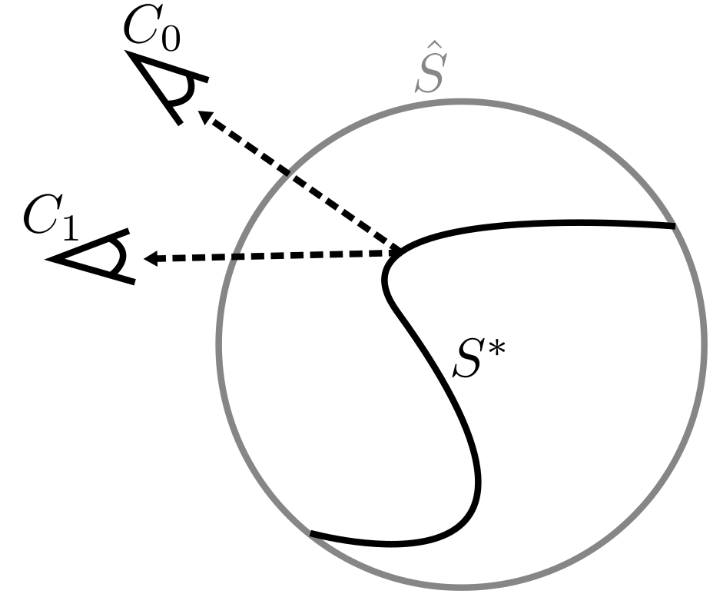
\includegraphics[width=0.6\textwidth]{undergraduate-thesis/images/omni-nerf/shape-radiance ambiguity.png}
    \caption{形状-辐射二义性示意图\cite{zhang_nerf_2020}}
    \label{fig:omni-nerf shape-radiance ambiguity}
\end{figure}

如图\ref{fig:omni-nerf shape-radiance ambiguity}所示,假设一个二维曲面$S^*$的形状为图中所示,相机$C_0, C_1$分别从不同角度观察曲面上一点,由图可以看出,如果网络实际学到的几何形状为图中$\hat{S}$所代表的单位圆,而将$C_0, C_1$观察到的颜色“贴”在单位圆上。这样即使网络学习到的几何与真实几何形状完全不同,也可以渲染出真实感的颜色。这种二义性被叫做“形状-辐射二义性”\cite{zhang_nerf_2020},因而由辐射场建模的场景几何通常被认为是欠约束的。

\subsection{解决方案}

为了解决这一问题,现有工作主要从两方面解决这一问题。其中一种方式是通过修改隐式场的内在结构,引入对场景几何结构更加敏感的符号距离场作为辐射场的前置组件,使用混合隐式场来构造场景表示。将符号距离场通过抽取符号距离函数$f_{SDF}(x)$的零值面来重建隐式表面。

另一种方式则是通过引入多元传感器信息输入作为额外监督信号。现有神经辐射场方法使用图片和其相机位姿作为网络输入,使用渲染颜色和真实观测颜色作为监督信号构建损失函数。通过反向传播损失函数值来优化多层感知机网络。注意到辐射场中的体积渲染方法同样可以用来计算累计深度值,为了改善该神经网络的表示精度,现有方法通过引入深度传感信息来构建额外的监督信号\cite{deng_depth-supervised_2022, roessle_dense_2022, azinovic_neural_2022}。

虽然这两种方法在一定程度上都可以弥补形状-辐射二义性,但目前的两种技术路线都不能在更大规模场景重建准确的场景几何。本文尝试将多元传感信息,特别是深度传感数据融入重建过程。然而,简单地使用深度误差优化混合隐式场存在二义性误差。首先分析将这两种技术路线相结合所带来的误差。并提出基于全方向距离场的混合隐式场景表征方法。

\section{混合隐式场内在误差}
符号距离场衡量了一个三维空间中的三维点到其最近表面的符号距离,而当符号距离函数被应用在体积渲染过程中时,通常需要显式地将距离函数值映射为体积密度或累计权重。本文以NeuralRGB-D\cite{azinovic_neural_2022}所提出的映射方案作为示例:
\begin{equation}
    w_i = \sigma\left(\frac{f_{TSDF}(t)}{\mathtt{trunc}}\right)\cdot\sigma\left(-\frac{f_{TSDF}(t)}{\mathtt{trunc}}\right),
    \label{eq: omninerf-basedline-weighting}
\end{equation}
其中$f_{TSDF}$为神经截断符号距离函数,这个映射将符号距离函数值映射为体积积分中的点权重,$\sigma$为任意选取的钟形单峰对称函数,这里使用$\mathtt{sigmoid}$函数。这个权重分配函数在一维上的可视化如图\ref{fig:omninerf-baseline-weighting}所示。

\begin{figure}[ht]
    \centering
    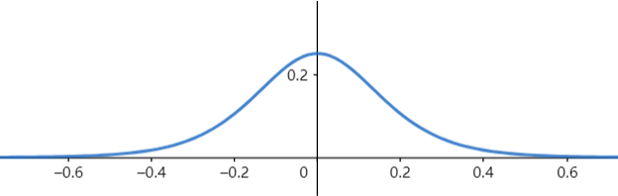
\includegraphics[width=0.6\textwidth]{undergraduate-thesis/images/omni-nerf/neural-rgbd weighting function.png}
    \caption{公式\ref{eq: omninerf-basedline-weighting}所计算的权重函数分布。}
    \label{fig:omninerf-baseline-weighting}
\end{figure}

通过公式可以看出,距离函数较小的值将被赋予更大的体渲染权重。当距离函数通过这一函数映射到点权重后,可以将体积渲染公式改写为:
\begin{equation}
    \hat{C}(r) = \frac 1 {\sum_{i=0}^{N-1}w_i}\sum_{i=0}^{N-1}w_i\cdot c_i
\end{equation}

\begin{figure}[t]
    \centering
    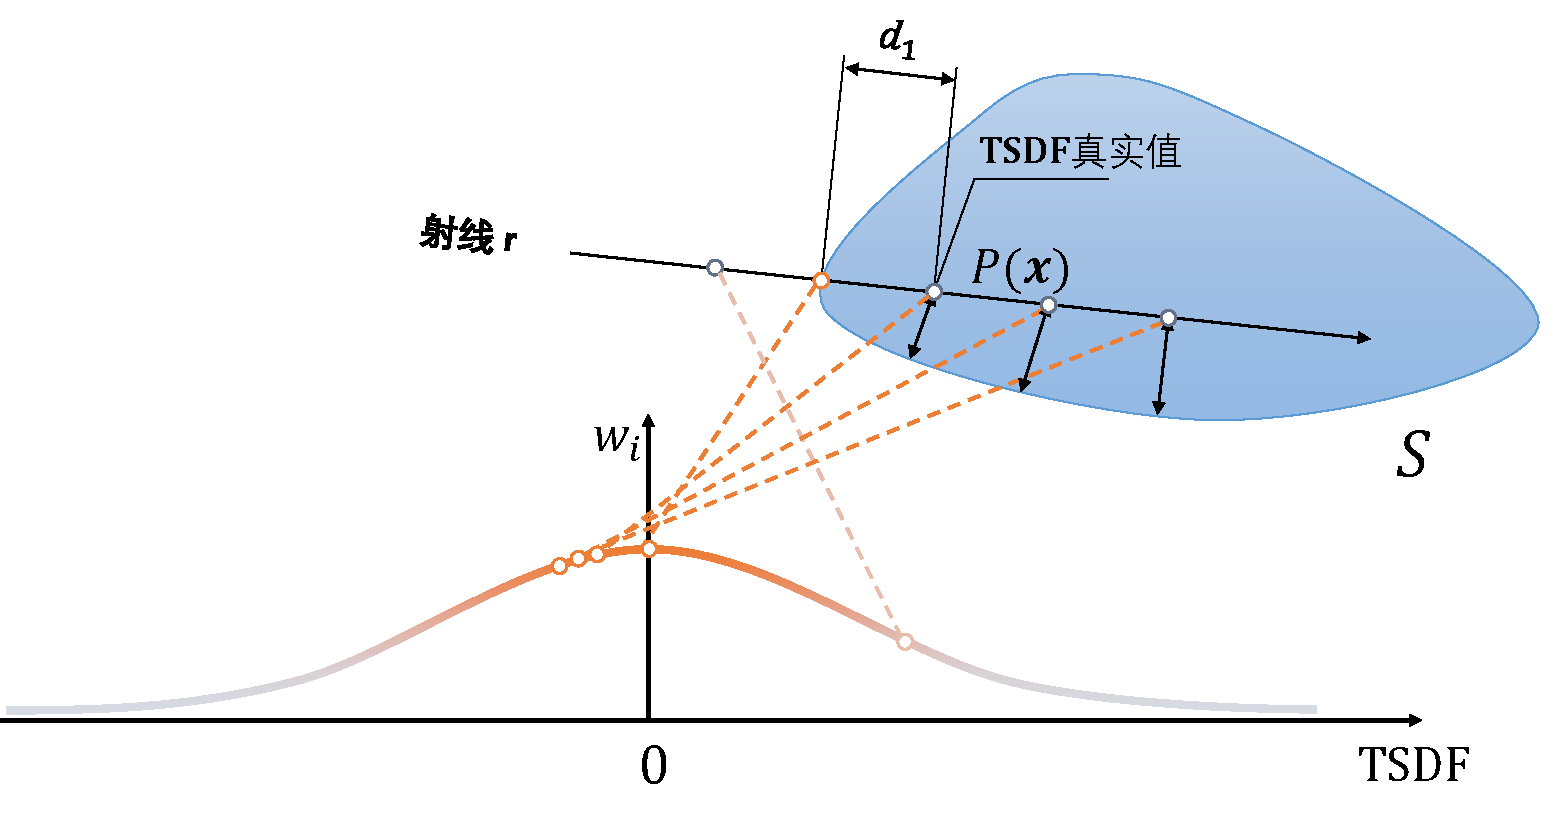
\includegraphics[width=\textwidth]{undergraduate-thesis/images/omni-nerf/omninerf-error2.pdf}
    \caption{混合隐式场内在误差的二维示意图}
    \label{fig:omninerf-internal error}
\end{figure}

在这样的框架下, 本文描述一种由混合隐式场方案引起的系统误差。对于隐式表面$\mathcal{S}$,假设发射的光线$\mathbf{r}(t)$与表面$\mathcal{S}$在$t=t_0,t_1$处分布相交($t_n<t_0<t_1<t_f$),且光线$\mathbf{r}(t)$在表面$\mathcal{S}$几乎相切处入射(如图\ref{fig:omninerf-internal error}所示)。

对于$t\in[t_0, t_1]$区间中的采样点$P(t_{k_1}), \dots, (t_{k_N})$,这些点由于均位于表面$\mathcal{S}$内部,因而在体积渲染过程中,应占有较小的权重。然而,由于光线沿表面入射,当表面较为光滑时,有:
\begin{equation}
    0\approx w(t_{k_i} - t_0) << w(f_{SDF}(t_{k_i})) \approx w(0),
\end{equation}
其中$w(t_{k_i} - t_0)$较好地反映了点$t_{k_i}$处的体积,而实际预测值$w(f_{SDF}(t_{k_i}))$远远大于该点的真实密度。

由于点$t_{k_i}$靠近曲面$\mathcal{S}$表面,因而在辐射场中,该点求得的辐射颜色接近于其最近表面点$p_{k_i} + \nabla f_{TSDF}(t_{k_i})\cdot f_{TSDF}(t_{k_i})$的颜色。从而在体渲染过程中产生颜色混淆的效果。
\begin{equation}
    \hat{c}(p_{k_i})\approx\hat{c}\left(p_{k_i} + \nabla f_{TSDF}(t_{k_i})\cdot f_{TSDF}(t_{k_i})\right)
\end{equation}


\section{结合深度输入的混合隐式场距离-深度二义性}
除了前文提到的使用混合隐式场作为场景表示时出现的隐式场内在误差,在本节中还将介绍使用深度信号作为混合隐式场监督信号时出现的距离-深度二义性。在第二章介绍了现有方法\cite{azinovic_neural_2022}在使用深度监督信号时在截断区域内所使用的深度损失函数:
\begin{equation}
    \mathcal{L}_{tr} = \sum_{p_{tr}}(f_{TSDF}(p_{tr})+t_{tr}-D)^2,
\end{equation}

该损失函数用$\hat{f}_{TSDF}(p_i) = D(\mathbf{r})-t_i$估计$p_i (p_i \in \mathbf{r})$点的截断符号距离函数。如图\ref{fig:omni-nerf depth error}所示,这个估计会对隐式场准确几何内容的学习产生很大的影响:当分别从两个视角$\mathbf{r}_1, \mathbf{r}_2$观察到同一空间点$P$时,由于该点到观察视角起点距离不同,由上述过程估计所得的对同一点的截断符号距离函数值$d_1, d_2$也不同,则当使用这两个不同的估计值同时作为点$P$的截断距离函数真值进行反向传播时,网络不能学到任意一个真实的TSDF值,从而导致结果模糊、计算资源浪费的结果。

\begin{figure}[ht]
    \centering
    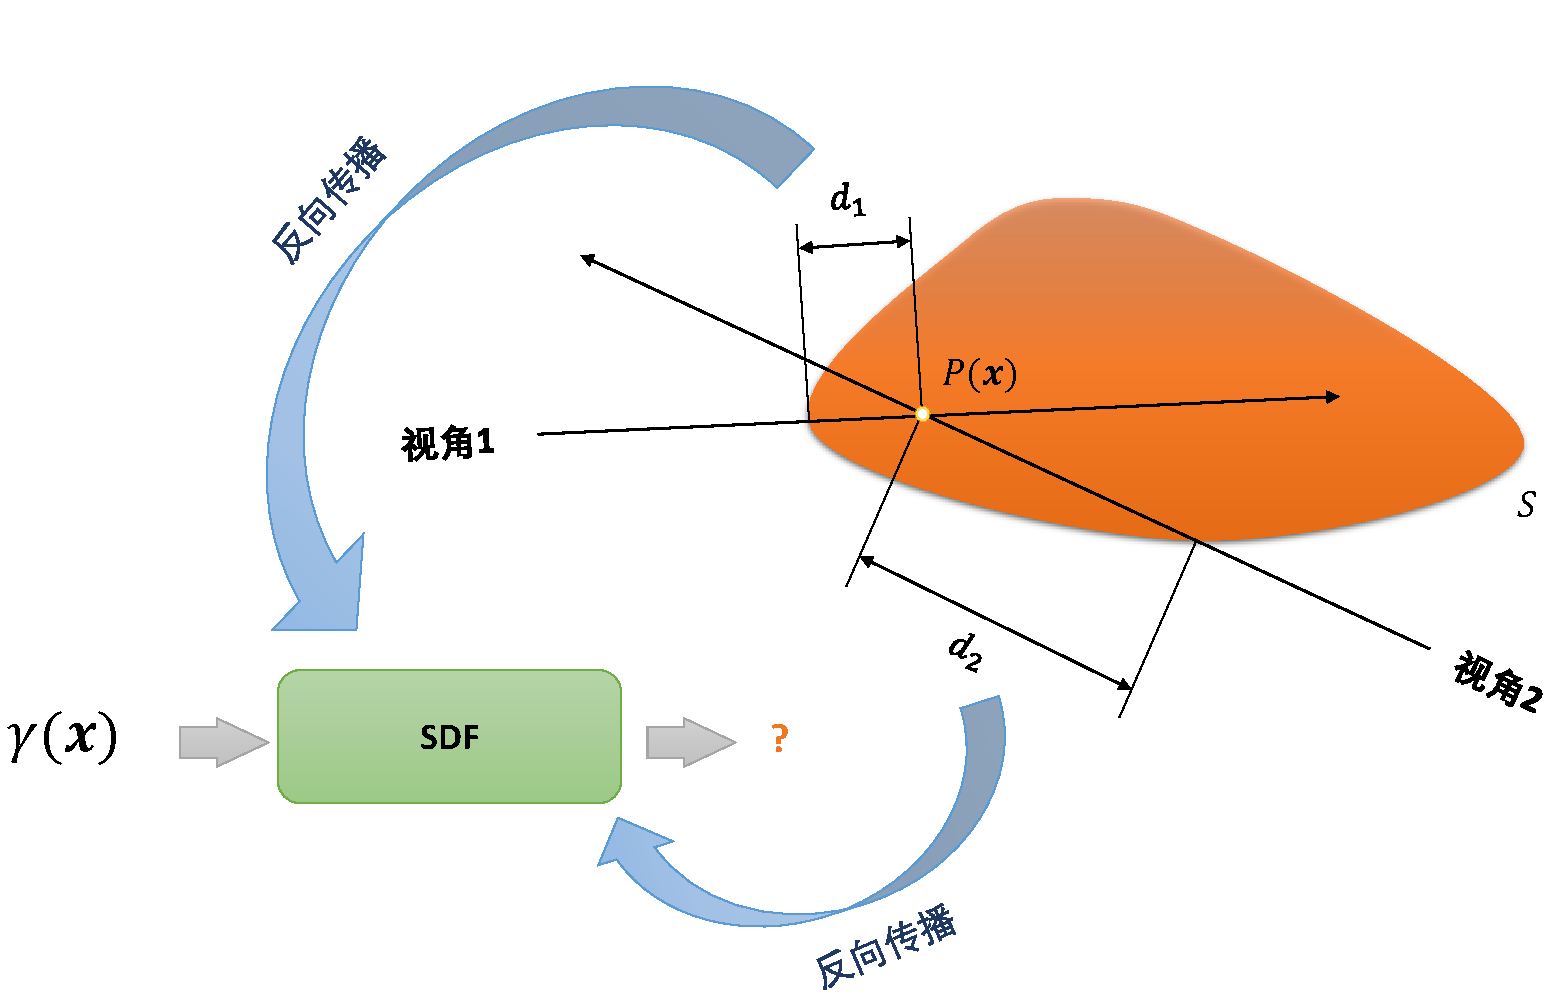
\includegraphics[width=\textwidth]{undergraduate-thesis/images/omni-nerf/omninerf-error1.pdf}
    \caption{深度监督信号下的混合隐式场二义性示意图。}
    \label{fig:omni-nerf depth error}
\end{figure}


\section{基于全方向距离场的混合隐式场表征}
通过分析上面提到的两种误差,本文发现他们都是由于现有基于符号距离场的混合隐式表征技术方案在距离场设计上没有考虑到多视角的视角相关性,即应该使用随视角方向变化的距离函数计算权重。

基于这一观察, 本文提出基于全方向距离场的混合隐式表征方案。全方向距离场(Omnidirectional Distance Field, ODF)接受位置和方向的五维输入数据$(x,y,z,\theta,\phi)$,输出视角相关的距离函数值。全方向距离函数值代表了空间点$\mathbf{x}=(x,y,z)$在方向$\mathbf{d}=(\theta,\phi)$上最近表面的无符号距离。
\begin{equation}
    f_{ODF}: (\mathbf{x},\mathbf{d})\to \mathbb{R}_+
    \label{eq: omninerf-odf function}
\end{equation}

注意到全方向距离函数可以分解为符号距离场和一个全方向距离残差函数的和:
\begin{equation}
    f_{ODF}(\mathbf{x}, \mathbf{d}) = |f_{SDF}(\mathbf{x})| + f_\Delta(\mathbf{x}, \mathbf{d})
    \label{eq: omninerf-odf decomposition}
\end{equation}

本文设计了如图\ref{fig:omninerf-model}所示的网络。输入$\mathbf{x}$首先通过符号距离场得到$\mathbf{x}$的符号距离,通过将网络输出的几何参数继续前传,同时输入观察方向$\mathbf{d}$,计算空间点的全方向距离残差函数值$f_\Delta(\mathbf{x},\mathbf{d})$和辐射颜色$\mathbf{c}_i$。

\begin{figure}[ht]
    \centering
    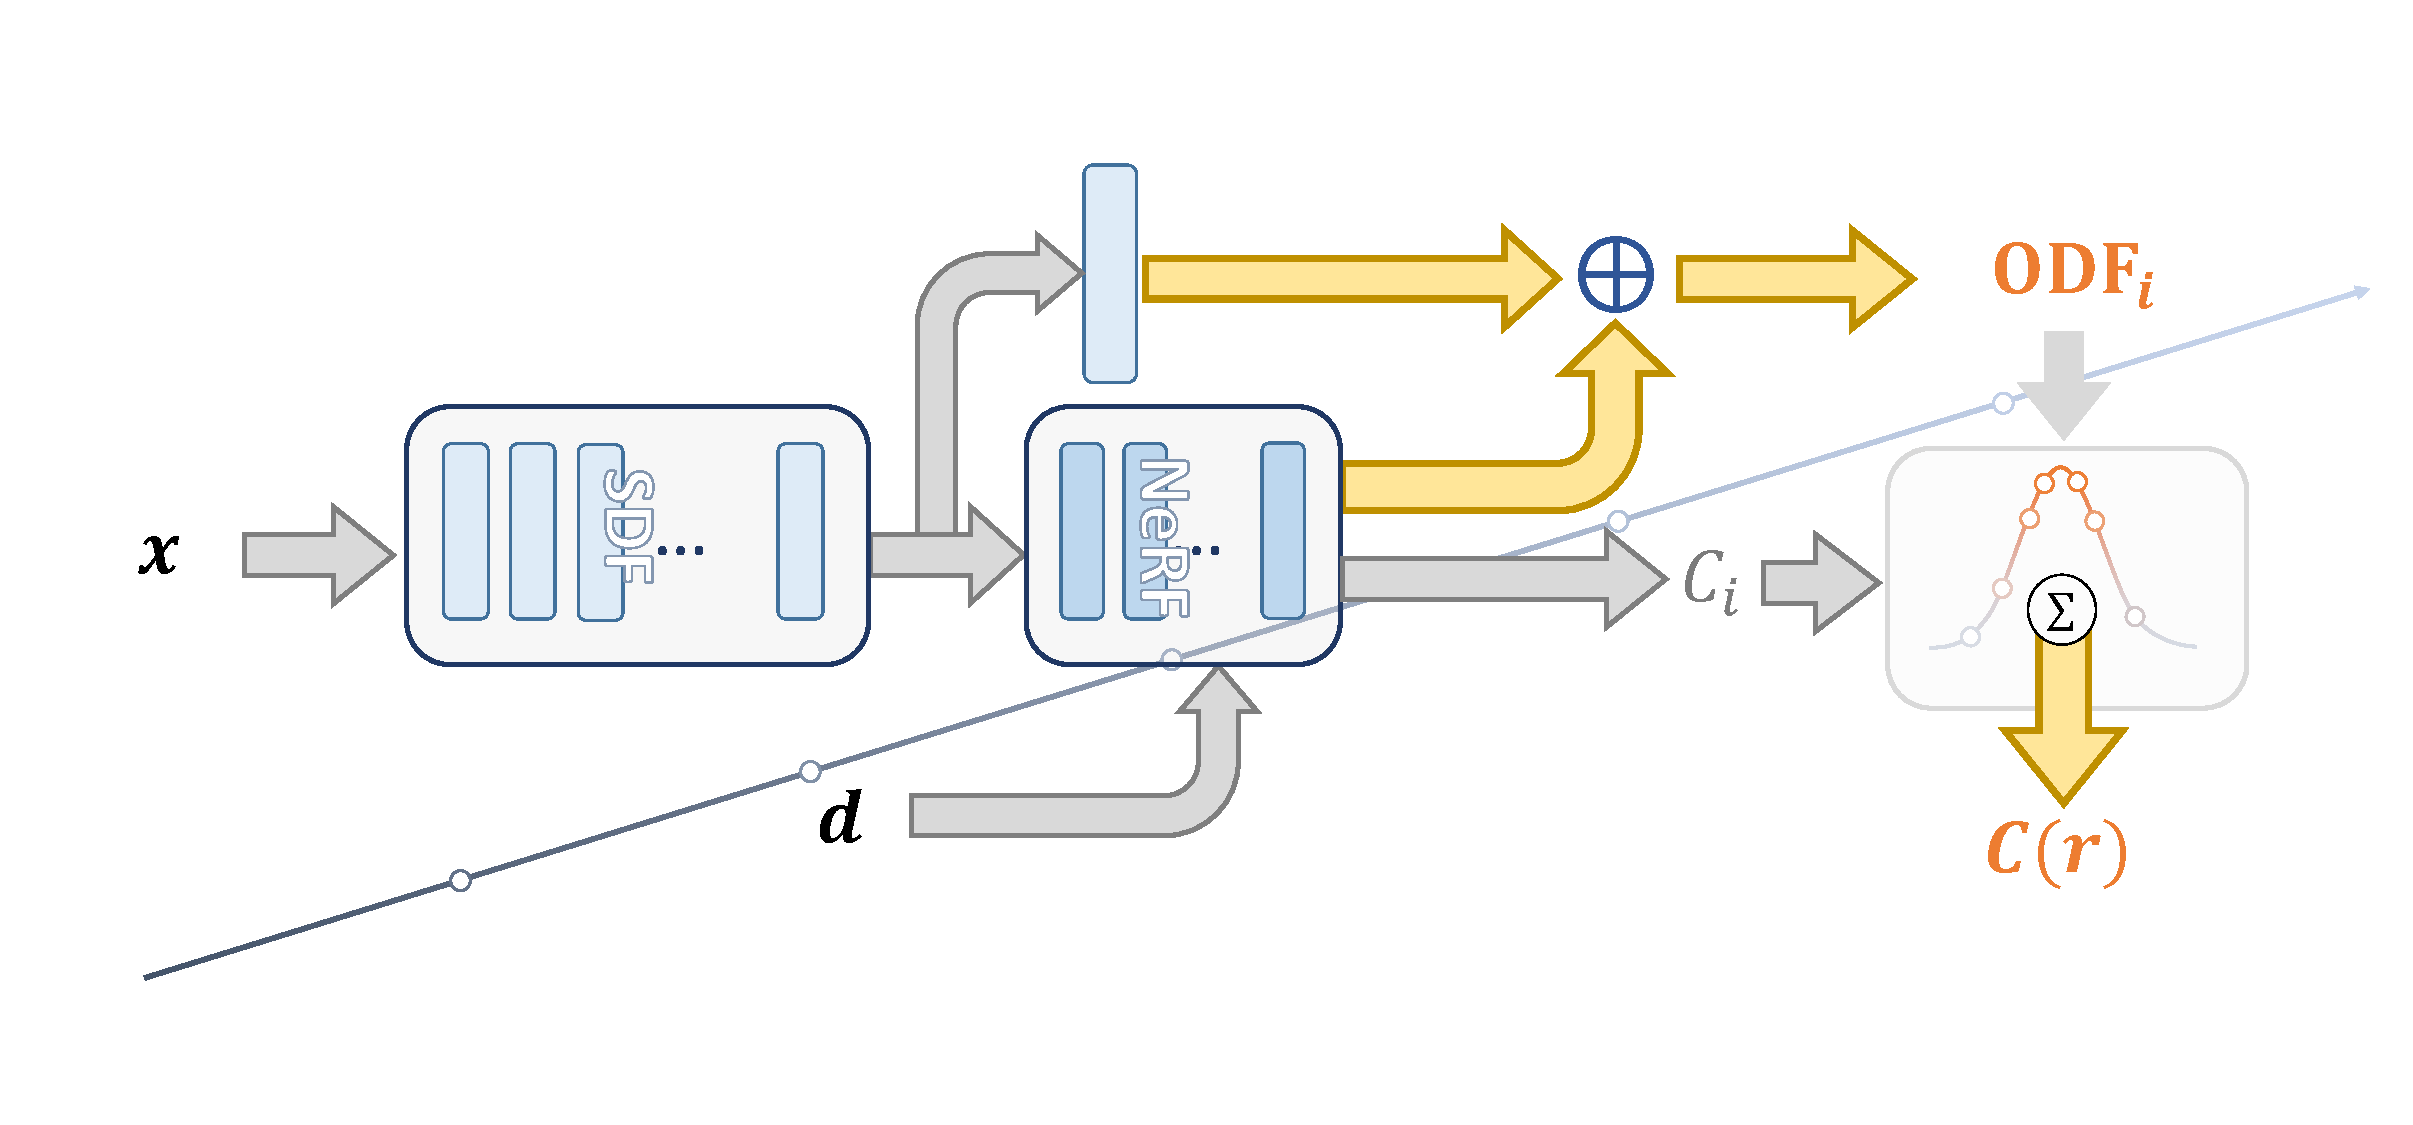
\includegraphics[width=\textwidth]{undergraduate-thesis/images/omni-nerf/omninerf-model.pdf}
    \caption{基于全方向距离场的混合隐式表征方案}
    \label{fig:omninerf-model}
\end{figure}

通过将符号距离函数和残差函数重新组合,便可以得到全方向距离函数值,将该值按照现有体积渲染方案经过积分,便可以在一条射线上得到渲染颜色$C(\mathbf{r})$。 可以验证,本文提出的混合隐式场融合方案可以从理论上解决混合隐式场的内在误差和深度监督后的距离-深度二义性。

\section{全方向混合隐式场景表示模型实现}
在前面几节中,本文基于两种现有方法中观察到的误差和二义性,在理论上提出了可以去除这两种误差的解决方案,本节详细描述使用全方向距离-辐射混合隐式场的实现方案。

在第\ref{chapter:related-work}章中介绍了现有的主流场景表示方法,其中,基于哈希体素网格的场景表示可以准确地建模场景细节但需要占据较大的存储空间。这些表示主要由于图形硬件限制而难以扩展到更大的场景。体积数据必然比 2D 表面表示更大并在内存中占用更多空间。类似地,虽然相机光线最多与硬表面相交一次,但渲染穿过体积的光线可能需要许多样本。使用神经或混合表示时,每一个采样在计算或内存带宽方面的评估都非常昂贵。因此,这类方法只适用于范围有限的场景(空间中的单个对象或Forward-Facing的场景)的方法通常不会扩展到更大的无界场景。而基于多平面的张量分解场景表示在准确性上有所下降,但可以用更低的存储空间达到相媲美的效果。本文结合这两种不同的场景表示,使用一个较低分辨率的哈希体素网格建模场景细节,并使用一个更高分辨率的多平面作为辅助,以达到高效的准确场景地图骨干模型。本文所提出方法的网络结构图如图\ref{fig:omninerf-scene-representation}所示。

\begin{figure}[ht]
    \centering
    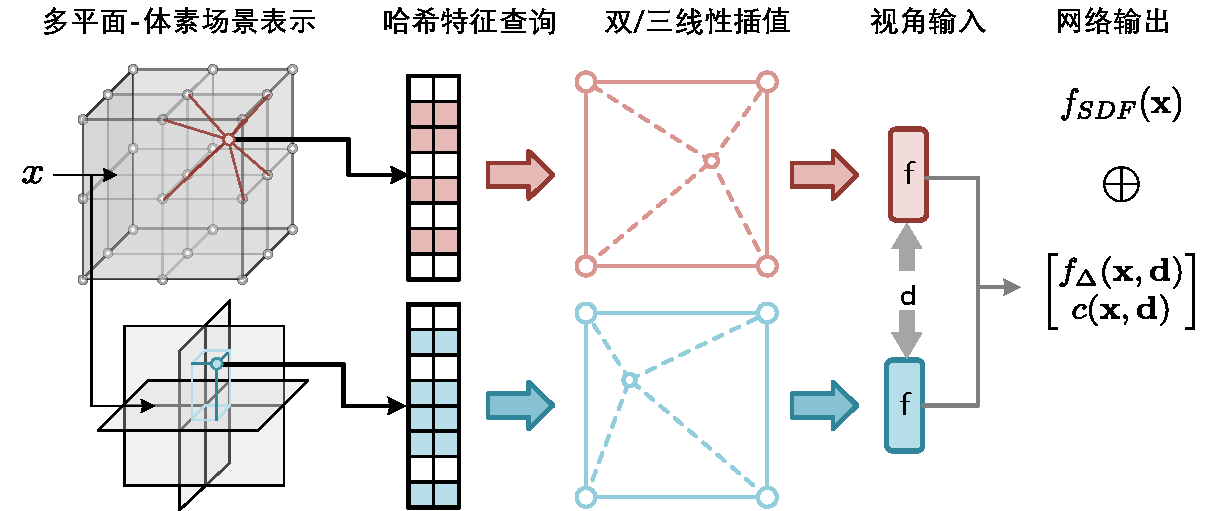
\includegraphics[width=\textwidth]{undergraduate-thesis/images/omni-nerf/omninerf-scene-representation.pdf}
    \caption{场景表示模型架构图}
    \label{fig:omninerf-scene-representation}
\end{figure}

对于任意输入三维点$\mathbf{x}$和观察视角$\mathbf{d}$,分别将三维点坐标输入多分辨率体素哈希网格$\{\mathcal{G}_l\}^L$和三平面$\mathcal{P}_{\{XY,XZ,YZ\}}$。

对于多分辨率体素哈希网格,通过在每一分辨率级别查询输点$\mathbf{x}$的八个相邻格点,将格点序号对应哈希函数(式\ref{eq: omninerf-hash functions})作为索引,获得每个格点对应的体素特征向量。通过三线性插值$\mathtt{interp}$在连续欧式空间下获得空间点$\mathbf{x}$处的体素特征。最后将每个分辨率层级获得的特征拼接,得到该点的输出特征向量$f_{\mathcal{G}}$。
\begin{equation}
    f_{\mathcal{G}} = \mathtt{concat}\{w_l(t)\cdot\mathtt{interp}(h^l(\mathbf{x}), \mathcal{G}_l)\}_{l=1}^L,
\end{equation}
这里$w_l$为逐层抗锯齿权重,本文将在第\ref{sec: omninerf-anti-aliasing}节描述该权重的设置。
\begin{equation}
    h^l(\mathbf{x}) = \left(\bigoplus_{i}x_i\pi_i^l\right) \text{mod}\ T,
    \label{eq: omninerf-hash functions}
\end{equation}
$T, \pi^l$为随机大质数。

对于三平面场景表示,首先将输入点$\mathbf{x}$投影到XY,XZ和YZ三个平面,接着对于每个投影坐标$\mathbf{x}_{XY},\mathbf{x}_{XZ},\mathbf{x}_{YZ}$,通过上下取整得到四个相邻格点序号,用将格点序号通过哈希函数获得的索引在哈希函数表中进行查找获得该点对应的体素特征向量,最后通过双线性插值得到分解后的三个特征向量:
\begin{equation}
    f_{plane} = \mathtt{interp}(h^{plane}(\mathbf{x}_{plane}), \mathcal{P}_{plane})
    ,plane=\{XY,XZ,YZ\}
\end{equation}

通过参数融合、拼接得到完整的特征向量。该特征向量可以被后续网络结构解码成为输出物理量:
\begin{equation}
    f(\mathbf{x}) = \mathtt{concat}\{f_{\mathcal{G}}, f_{XY}\otimes f_{XZ} \otimes f_{YZ}\},
\end{equation}
这里$\otimes$为Hadamard乘积\cite{fridovich-keil_k-planes_2023}。

为了鼓励空间平滑和连贯性,本文中使用的模型包含不同空间分辨率的多个副本,如: 64、128、256 和 512。每个尺度的模型都将被单独处理,来自不同尺度的特征向量被连接在一起,并传递给后续步骤。受 InstantNGP \cite{muller_instant_2022} 的多尺度哈希映射的启发,这种表示有效地编码了不同尺度的空间特征,能够减少以最高分辨率存储的特征数量,从而进一步压缩模型。

通过参数解码器和激活函数,可以获得该点的无符号距离函数值:
\begin{equation}
    |f_{SDF}(\mathbf{x})| = \mathtt{activate}(f_{SDF}(f(\mathbf{x}))),
\end{equation}
其中,激活函数$\mathtt{activate}(x)=|x|$,参数解码器$f_{SDF}$为一个浅层的多层感知机。

接下来,网络会结合观察角度$\mathbf{d}$求得残差距离$f_\Delta(\mathbf{x}, \mathbf{d})$和辐射颜色$\mathbf{c}(\mathbf{x},\mathbf{d})$:
\begin{align}
    f_\Delta(\mathbf{x}, \mathbf{d})&=f_\Delta(f(\mathbf{x}), \gamma(\mathbf{d}))\\
    \mathbf{c}(\mathbf{x},\mathbf{d}) &=f_c(f(\mathbf{x}), \gamma(\mathbf{d}))
\end{align}

基于求得的无符号距离和全方向距离残差,通过公式\ref{eq: omninerf-odf decomposition}获得全方向距离函数值,该函数值进而通过下式中的权重函数被转换为体渲染权重:
\begin{equation}
    w(\mathbf{x},\mathbf{d}) = \mathtt{sigmoid}\left(\frac{f_{ODF}(\mathbf{x},\mathbf{d})}{\mathtt{trunc}}\right)\cdot\mathtt{sigmoid}\left(-\frac{f_{ODF}(\mathbf{x},\mathbf{d})}{\mathtt{trunc}}\right)
\end{equation}

对于射线$\mathbf{r} = (\mathbf{o},\mathbf{d})$的采样点集合$\{P_i\}_{i=0}^{N-1}$,对每个点$\mathbf{x}_i=\mathbf{o}+t_i\mathbf{d}$获得其全方向距离值$\{f_{ODF}(\mathbf{x}_i,\mathbf{d})\}^N$和辐射颜色$\mathbf{c}(\mathbf{x}_i,\mathbf{d})$,通过体渲染公式求得渲染点颜色和深度:
\begin{align}
    \mathbf{C}(\mathbf{r}) &= \sum_{i=0}^{N-1}w(\mathbf{x}_i,\mathbf{d})\mathbf{c}(\mathbf{x}_i,\mathbf{d})\\
    D(\mathbf{r}) &= \sum_{i=0}^{N-1}w(\mathbf{x}_i,\mathbf{d})\cdot t_i
\end{align}

\subsection{基于Proposal网络的采样策略}
本文与大部分体渲染方法一样,在渲染过程中需要使用有限的采样对体渲染积分进行近似。在本文中使用基于Proposal网络的分层采样策略。即使用一个轻量级网络,从空间点坐标估计体密度$\hat{\sigma}(\mathbf{x})$:
\begin{equation}
    f_{Proposal}:\quad \mathbf{x}\to\hat{\sigma}(\mathbf{x})
\end{equation}

Mip-NeRF\cite{barron_mip-nerf_2021}使用从粗到精的重采样策略,其中 MLP 使用“粗”射线间隔评估一次,然后使用“精细”射线间隔再次评估,并在两个级别上使用图像重建损失进行监督。本文在此基础上进行了改进,使用两个MLP:一个NeRF场景表示模型,以及一个Proposal网络,其中Proposal网络根据输入空间坐标预测体密度,被用来作为重采样的基准。

\begin{figure}[ht]
    \centering
    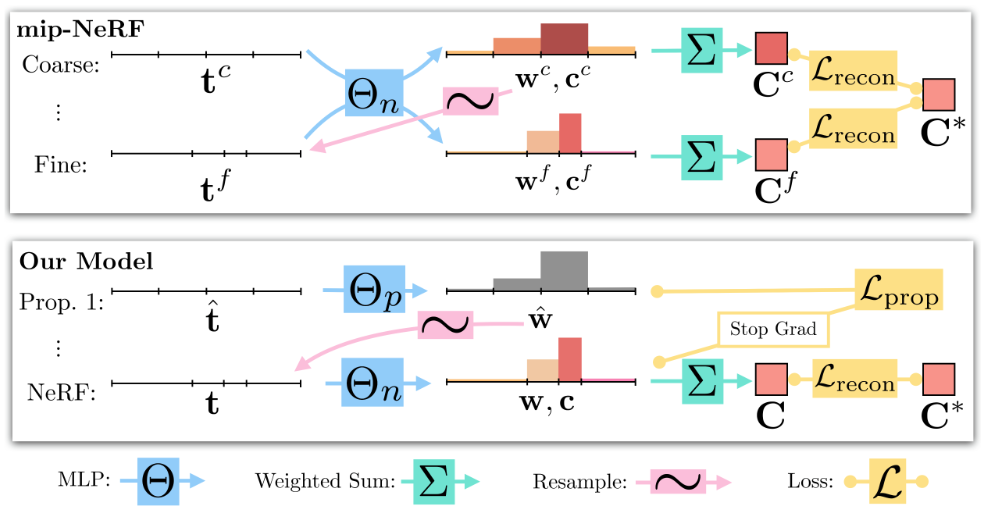
\includegraphics[width=\textwidth]{undergraduate-thesis/images/omni-nerf/mip-nerf360 proposal network.png}
    \caption{Proposal网络结构示意图。}
    \label{fig:related-work proposal network}
\end{figure}

如图\ref{fig:related-work proposal network}所示,Mip-NeRF 使用一个多尺度 MLP,该 MLP 被反复查询来获取权重,这些权重被重新采样到下一阶段的间隔中,并监督在所有尺度上生成的渲染。Mip-NeRF 360使用“Proposal MLP”,在渲染阶段,使用“NeRF MLP”来生成权重和颜色来渲染图像。Proposal MLP 被训练以产生与 NeRF MLP 的 w 输出一致的Proposal权重$\hat{w}$。通过使用小型Proposal MLP 和大型 NeRF MLP,Mip-NeRF 360获得了一个具有高容量且易于训练的组合模型。

\subsubsection{基于重要性的重采样方法}

本文会首先进行从相机原点$t_n$到假想无穷远点$t_f$的归一化空间中均匀采样:
\begin{equation}
    s_i\sim\mathcal{U}\left[\frac{i-1}{N}, \frac{i}{N}\right],
\end{equation}
$s_i\in(0,1]$为点的归一化深度,本文通过下面的方式计算归一化深度:
\begin{align}
    s_i&:=\frac{g(t_i)-g(t_n)}{g(t_f)-g(t_n)}\\
    t&=g^{-1}(s\cdot g(t_f) + (1-s)\cdot g(t_n))\\
    g(t)&:= 1/x
\end{align}

采样得到粗采样的$N_c$个点的点集$\{t_i^c\}_{i=1}^{N_c}$会被输入到$f_{Proposal}$网络中查询所对应的体积密度$\{\hat{\sigma}(t_i^c)\}^{N_c}$,通过体积渲染方法计算这些点的权重:
\begin{equation}
    w_i^c = \frac{T_i(1-\exp(-\hat{\sigma}(t_i^c)\delta_i^c))}{\sum_j w_j^c},
\end{equation}
其中$\delta_i^c = t_{i+1}^c - t_i^c$为采样区间长度。$w_i^c = \text{PDF}_i$可以看作为射线上点权重分布的概率密度函数。

根据算得的概率密度函数,可以进行基于概率分布的重新采样,即在更高权重的地方放置更多采样点。这里首先计算累计分布值:
\begin{equation}
    \text{CDF}_i = \sum_{j \leq i} \text{PDF}_i
\end{equation}

通过在累计分布函数的逆函数$\text{CDF}^{-1}$上进行均匀采样,即可获得重新采样后的$N_f$个精采样点$\{t_i^f\}_{i=1}^{N_f}$,精采样点会被作为最终采样点输入到场景表达中进行体积渲染:
\begin{align}
    s^f_i &= \text{CDF}^{-1}(1/(i + 1))\\
    t^f_i &= g^{-1}(s^f_i\cdot g(t_f) + (1-s^f_i)\cdot g(t_n)
\end{align}

\subsubsection{基于知识蒸馏的Proposal网络优化}

Proposal网络的训练需要通过从场景表达网络中蒸馏得到,注意到粗采样和精采样的采样区间并不一定相同,因而对蒸馏训练带来了一定的困难,本文中使用覆盖损失函数的方式优化Proposal网络\cite{barron_mip-nerf_2022}。即对所有与查询区间$<t_{j}^f, t_{j+1}^f>$有交的粗采样区间,计算所有满足条件的粗采样区间权重的和。
\begin{equation}
    \mathtt{bound}(\{t_i^c\}_{i=1}^{N_c}, \{w_i^c\}_{i=1}^{N_c}, <t_{j}^f, t_{j+1}^f>) :=\sum_{k:<t_{k}^c,t_{k+1}^c>\cap<t_{j}^f, t_{j+1}^f>\neq\varnothing}\hat{w}_k^f
\end{equation}

对于任意一个精采样区间$<t_{j}^f, t_{j+1}^f>$,当满足$w_j^f\leq \mathtt{bound}(\{t_i^c\}_{i=1}^{N_c}, \{w_i^c\}_{i=1}^{N_c}, <t_{j}^f, t_{j+1}^f>)$时,则Proposal网络与场景表示网络的分布相同。因此可以利用$\mathtt{bound}$函数设计损失函数:
\begin{equation}
    \mathcal{L}_{Proposal}=\sum_j\frac{1}{w_j^f}\max(0, w_j^f- \mathtt{bound}(\{t_i^c\}_{i=1}^{N_c}, \{w_i^c\}_{i=1}^{N_c}, <t_{j}^f, t_{j+1}^f>))^2
\end{equation}

\subsection{优化全方向距离-辐射隐式场}
为了优化全方向距离-辐射混合隐式场,本文设计了如下的损失函数:
\begin{equation}
    \mathcal{L} = \lambda_{color}\mathcal{L}_{color} + \lambda_{depth}\mathcal{L}_{depth}+\lambda_{ODF}\mathcal{L}_{ODF}+\lambda_{Proposal}\mathcal{L}_{Proposal},
\end{equation}
其中$\lambda_{\Box}$为对应损失函数项的权重。

在渲染颜色、深度的损失函数设计上,本文沿用现有方法\cite{mildenhall_nerf_2020}中较为常用的光度和深度误差:
\begin{align}
    \mathcal{L}_{color} &= \sum_{\mathbf{r}}||\hat{C}(\mathbf{r}) - C(\mathbf{r})||_2^2\\
    \mathcal{L}_{depth} &= \sum_{\mathbf{r}}||\hat{D}(\mathbf{r}) - D(\mathbf{r})||_2^2
\end{align}

对于全方向距离场,本文从输入深度图中估计采样点全方向距离函数值,并使用Eikonal约束\cite{gropp_implicit_2020}共同组成损失函数:
\begin{align}
    \mathcal{L}_{ODF} &= \sum_{\mathbf{r}}\sum_{i=1}^{N_f}||f_{ODF}(\mathbf{x}_i^f, \mathbf{d}) - \text{ODF}_i^{\mathbf{r}}||_2^2 + (||\nabla f_{ODF}(\mathbf{x}_i^f, \mathbf{d})||_2-1)^2\\
    \text{ODF}_i^{\mathbf{r}} &= |D(\mathbf{r}) - t_i^f|
\end{align}

\section{基于网格场景表示的抗锯齿渲染}
\label{sec: omninerf-anti-aliasing}
第\ref{chapter:related-work}章介绍了使用集成位置编码的抗锯齿渲染方法\cite{barron_mip-nerf_2021, barron_mip-nerf_2022},然而对于体素网格、多平面的场景表示,位置编码、集成位置编码均不再适用:由于PE/IPE的输出维度$2L+1$($L>5$)较高,如果构造一个高维的体素网格(即空间复杂度为$\mathcal{O}(N^{2L+1}$),将会对存储开销带来极大的负荷。

本文中利用传统计算机图形学中MipMap\cite{williams_pyramidal_1983}的思想,将其迁移在网格类场景表示中,通过设计一个新型采样点权重函数来解决锯齿问题。

在传统图形渲染管线中,当使用同一张高分辨率的材质图片渲染不同远近的物体时,会出现“摩尔纹”等瑕疵现象,为了解决这一问题,通常会使用MipMap的方法,即预先计算出同一物体材质贴图的不同分辨率下的一组“金字塔”。当观察物体距离相机起点较远时,使用更小分辨率的贴图进行采样,而当观察近处物体时,为了获得更多纹理细节, 则采用更大分辨率的贴图进行采样。这样做的原因是当从远处观察一个物体时,单个像素所覆盖的物体区域较大,此时使用高分辨率贴图进行渲染容易采样到物体表面的高频纹理细节,使用低分辨率的贴图从统计上可以理解为在像素所覆盖区域进行了超采样。

注意到多分辨率体素网格本身可以被看作场景的MipMap,为了在体素网格中模拟MipMap的效果,本文通过设计一个权重函数$w_l(t)$使距离相机较近($t\approx t_n$)使用分辨率较高的体素网格,而使较远的采样点使用分辨率较小的网格。对于$L$级多分辨率体素网格,本文通过一组一维高斯函数建模权重函数:
\begin{equation}
    w_l(t) = \mathtt{activate}(\frac{1}{\sqrt{2\pi}\sigma_l}\exp(-\frac{(t-t_l)^2}{2\sigma_l^2})),
\end{equation}
其中$\mathtt{activate}(x) = \mathtt{sigmoid}(x)$, $t_l, \sigma_l$为第$l$级体素网格所使用高斯分布的均值和标准差:
\begin{align}
    t_l &:= g^{-1}(s_l\cdot g(t_f) + (1-s_l)\cdot g(t_n)\\
    s_l &:= \frac{l + 1}{1 + L}\\
    \sigma_l &:= t_{l+1} - t_{l}
\end{align}


\section{本章小结}
本章介绍了一种新型混合神经隐式场的表征方法。 在现有方法中存在距离-辐射场的内在和距离-深度二义性误差,为了解决这些问题,本文提出使用基于全方向距离场的混合隐式场,可以证明本文提出的方法中上述误差不再存在。为了进一步提升渲染质量,在本章中还结合多种场景表示,使用Proposal网络进行采样,并在基于网格的场景表示中引入抗锯齿渲染技术。